\chapter{Applicazione contraffatta}

\section{Introduzione}

In questa sezione verrà illustrato un possibile attacco, eseguito sull'applicazione testata, che permette di ottenere il controllo totale sul dispositivo vittima. Verrà infatti creata una versione dell'applicazione indistinguibile dall'originale, ma contenente un trojan che instaurerà una connessione remota con l'attaccante permettendogli così l'accesso al dispositivo.

Di seguito, il procedimento per effettuare questo tipo di attacco.

\section{Esecuzione}

\begin{figure}[h]
	\centering
	\fbox{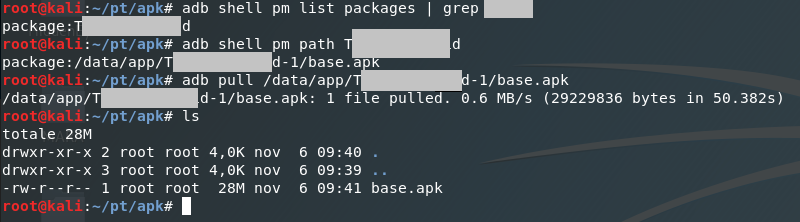
\includegraphics[width=.9\textwidth]{app/apk}}
	\caption{Ottenimento apk.}
	\label{fig:apk}
\end{figure}

L'unica cosa di cui si ha bisogno è l'apk originale. Esso può essere ottenuto in svariati modi. In questo caso è stato preso direttamente dal dispositivo della vittima tramite adb (figura \ref{fig:apk}).

Una volta ottenuto l'apk, utilizziamo \emph{msfvenom}\cite{MSFVenom} per iniettare la backdoor. Il comando viene lanciato indicando come payload da iniettare una connessione \emph{meterpreter}$/$\emph{reverse-tcp} chiedendo di instaurare la connessione all'IP $10.10.50.50$ (l'indirizzo del computer dell'attaccante).

Come si può vedere nella figura \ref{fig:backdoor}, \emph{msfvenom} riconosce automaticamente la piattaforma (Android) e l'architettura (Dalvik) ed esegue i seguenti passi:

\begin{itemize}
	\item Crea una \emph{signing key} ed un \emph{keystore} che verranno utilizzati per firmare la nuova applicazione modificata.
	\item Decompila l'apk originale.
	\item Decompila l'apk del payload.
	\item Analizza il codice e localizza il punto nel quale iniettare il malware.
	\item Inietta il malware collegandolo alla activity principale.
	\item Aggiunge i permessi necessari a prendere il controllo del dispositivo.
	\item Effettua la build del nuovo apk.
	\item Allinea e firma con le chiavi create in precedenza il nuovo apk.
\end{itemize}

\begin{figure}[h]
	\centering
	\fbox{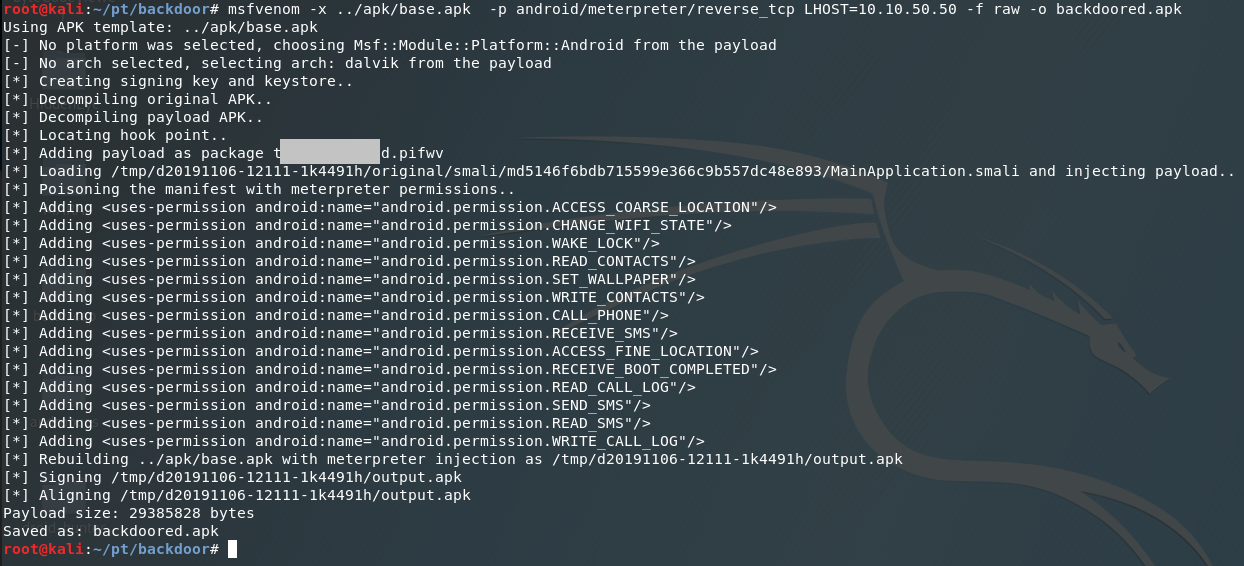
\includegraphics[width=.9\textwidth]{app/backdoor}} 
	\caption{Creazione backdoor.}
	\label{fig:backdoor} 
\end{figure}

Dopo aver creato l'applicazione malevola, l'attaccante lancia un server \ac{CC} tramite la piattaforma \emph{metasploit} (figura \ref{fig:metasploit}) ed inizia ad aspettare connessioni sulla porta $4444$. È possibile configurare l'exploit in modo che accetti connessioni dirette alla porta $4444$ da uno specifico IP (se conosciamo esattamente l'IP della vittima) o da qualunque IP (questa funzione si rivela molto utile in caso di IP dinamici).

\begin{figure}[h]
	\centering
	\fbox{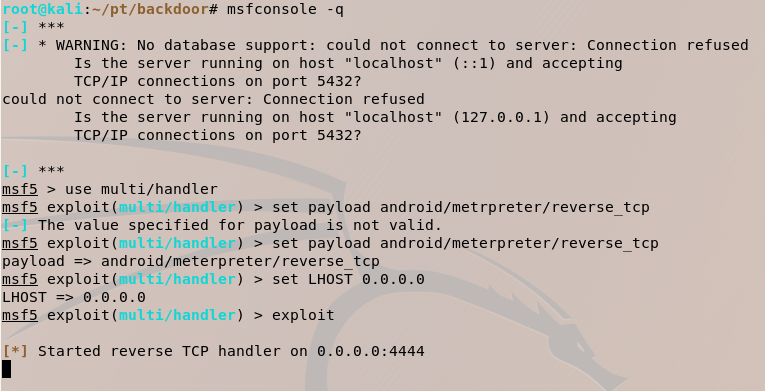
\includegraphics[width=.9\textwidth]{app/metasploit}} 
	\caption{Server C\&C.}
	\label{fig:metasploit} 
\end{figure}

Fino a questo punto non c'è stato bisogno di interagire con la vittima ed è stata creata tutta la struttura dell'attacco in maniera quasi automatica. L'intero processo non ha richiesto alcuna informazione oltre all'apk originale.

Adesso bisogna sfruttare la componente notoriamente più debole nell'ambito della cybersecurity: l'utente.

L'attaccante deve infatti convincere la vittima a scaricare ed installare l'applicazione contraffatta (supponendo che non abbia direttamente a disposizione il dispositivo, nel qual caso può provvedere direttamente all'installazione).

Il metodo migliore per ottenere questa collaborazione è sicuramente tramite operazioni di social-engineering. L'attaccante può ad esempio mandare una email alla vittima nella quale si richiede di aggiornare con la massima urgenza l'applicazione a causa di problemi di sicurezza. L'apk malevolo potrebbe essere spedito come allegato della mail insieme alle istruzioni su come installarlo. Un altro metodo potrebbe essere quello di fornire un link dal quale scaricare l'apk malevolo come si vede in figura \ref{fig:server}.

\begin{figure}[h]
	\centering
	\fbox{
		\subfloat[Download.]{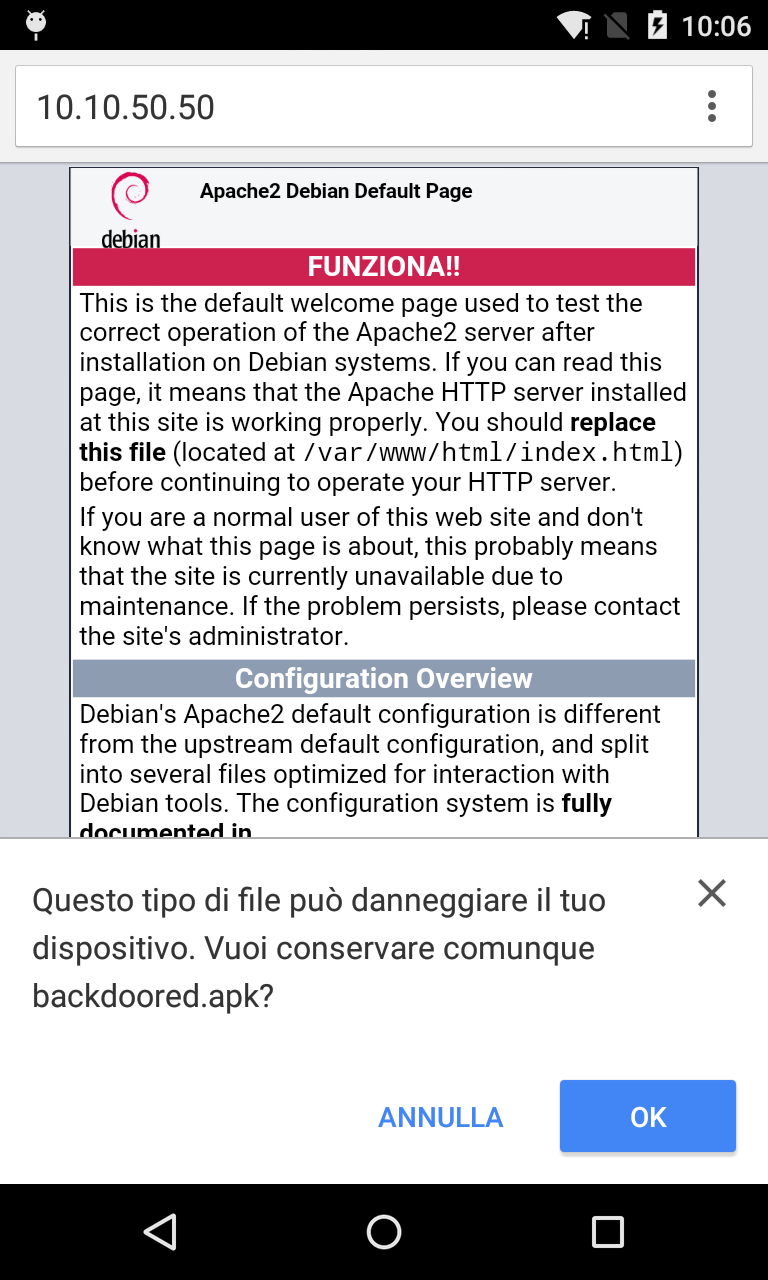
\includegraphics[width=.3\textwidth]{app/download}\label{fig:server}} \quad
		\subfloat[Installazione.]{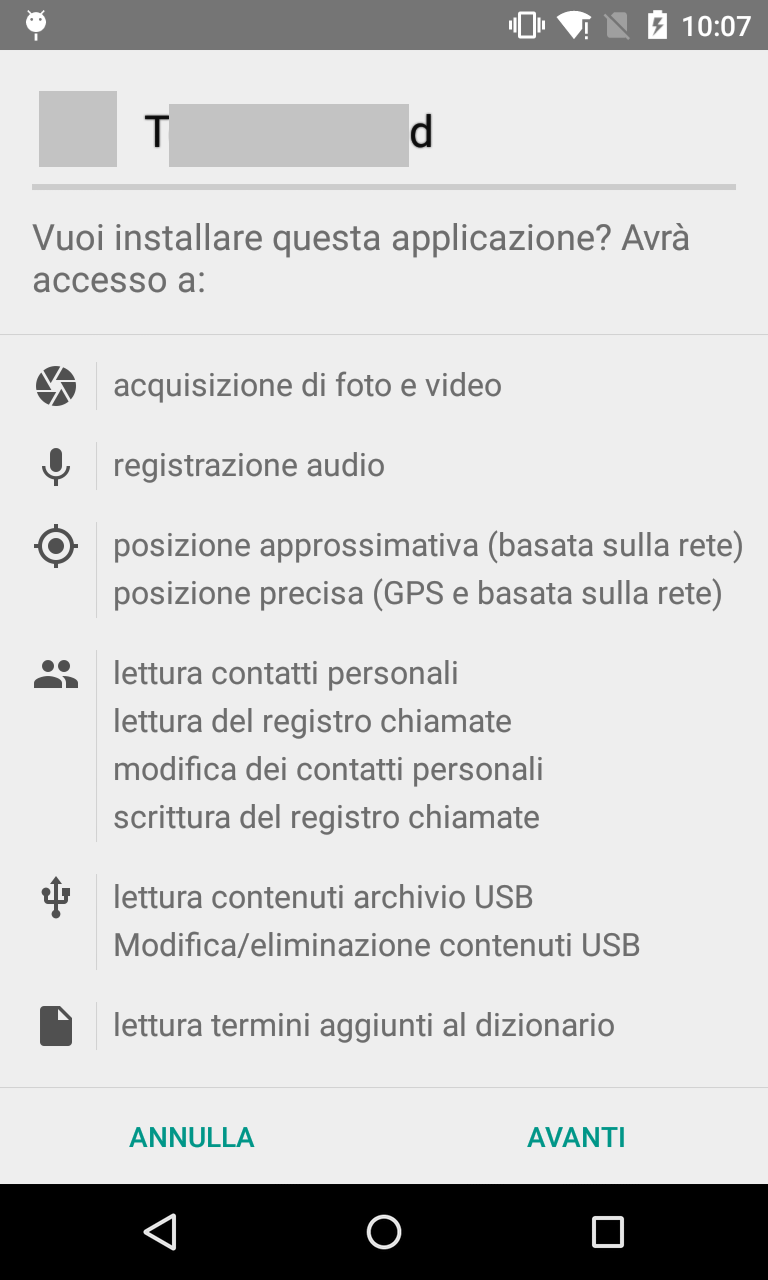
\includegraphics[width=.3\textwidth]{app/installazione}} \quad
		\subfloat[Applicazione.]{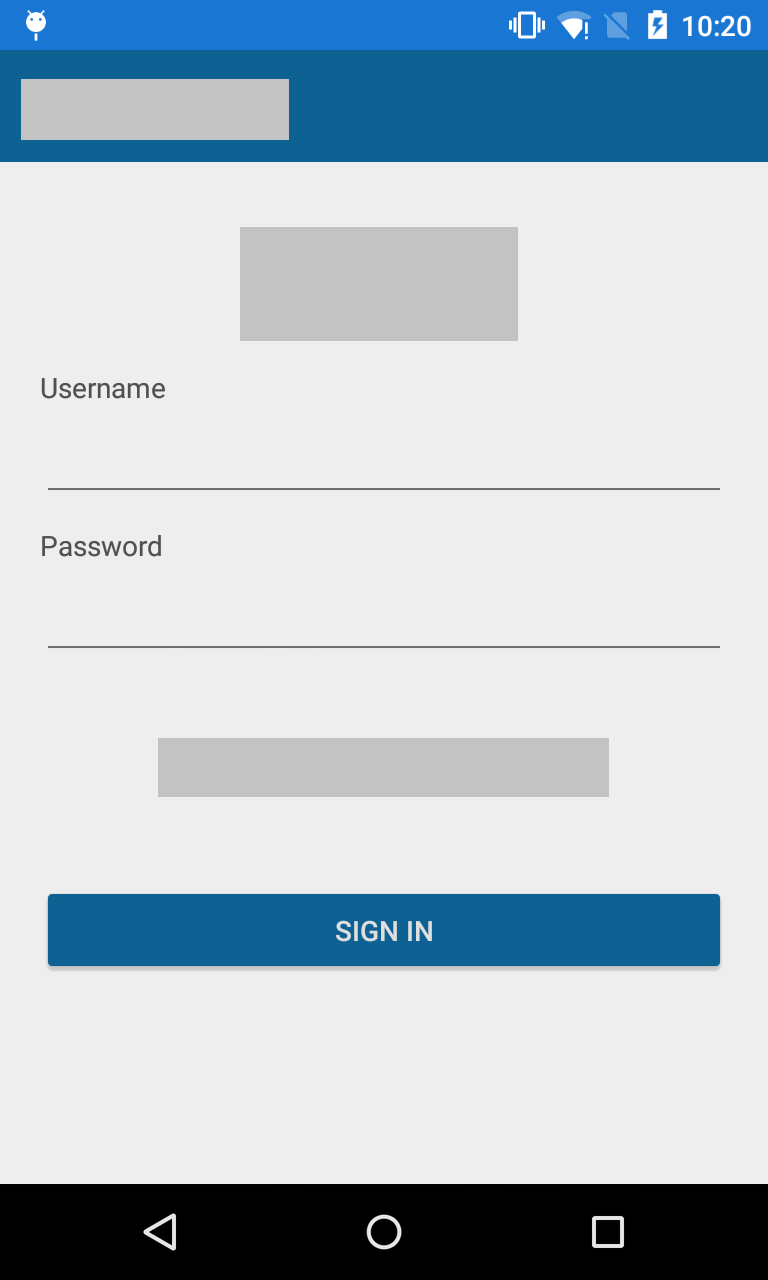
\includegraphics[width=.3\textwidth]{app/applicazione}\label{fig:grafica}}
	}
	\caption{Operazioni lato vittima.}
\end{figure}

Come si può vedere, l'applicazione installata è indistinguibile dall'originale sia come grafica (figura \ref{fig:grafica}) che come utilizzo in quanto non sono state apportate modifiche alle funzionalità della stessa. 

Nel momento in cui viene lanciata la prima volta, viene contattato il server \ac{CC} sulla porta $4444$, viene creata la connessione, si apre una sessione \emph{meterpreter} (figura \ref{fig:meterpreter}) e l'attaccante ha accesso al dispositivo vittima. Adesso è possibile scaricare l'elenco dei contatti, dei messaggi, delle foto e video, registrare audio, effettuare screenshot, scattare foto e registrare video tramite la fotocamera. Una volta ottenuto l'accesso al dispositivo è anche possibile installare in autonomia altre applicazioni malevole utili all'attaccante per aumentare il proprio potere di controllo sul dispositivo. Tutte queste operazioni vengono eseguite in maniera perfettamente trasparente alla vittima che non ha modo di accorgersi di quello che sta succedendo. 

È da notare il fatto che questa connessione sopravvive alla chiusura dell'applicazione e viene reinstaurata anche dopo un riavvio del dispositivo il quale risulta compromesso in maniera quasi irreversibile.

\begin{figure}[h]
	\centering
	\fbox{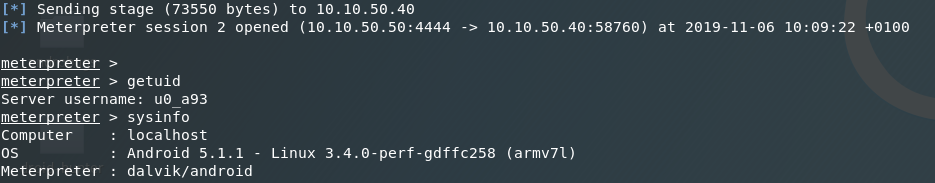
\includegraphics[width=.9\textwidth]{app/meterpreter}} 
	\caption{Connessione col server C\&C.}
	\label{fig:meterpreter} 
\end{figure}

\section{Soluzione}

Per quanto quella appena descritta non sia una vulnerabilità specifica dell'applicazione sotto analisi, è comunque importante rendere consapevole l'utente finale di questo rischio ed istruirlo a non installare mai applicazioni provenienti da sorgenti non sicure.

L'offuscamento del codice potrebbe rendere più difficile la decompilazione e la modifica dell'apk originale mitigando parzialmente questo tipo di problema ma la protezione totale è purtroppo impossibile da ottenere.